% !TeX root = ../../thesis.tex
\chapter{Introduction}\label{ch:introduction}

\section{Semiconductor Image Sensors}

Semiconductor image sensors have become an essential commodity of modern life, seamlessly integrated into consumer electronics. Yet their impact extends far beyond, finding vital applications in medical imaging, scientific research, automotive systems, industrial surveillance, and quality control \cite{Shi2023ApplicationsInnovations}. As of 2024, image sensors accounted for 4\% of the total semiconductor industry, generating over \$20 billion revenue \cite{Domengie2024TheApplications}. Nearly 90\% of these sales came from complementary metal oxide semiconductor (CMOS) image sensors, which became the dominant technology only as of 2010, taking over their predecessor, the charge-coupled device (CCD) image sensors. The dominance of the CMOS image sensor has been attributed to their cost-effective and large-scale production in standard foundries, combined with their superior efficiency in power consumption and high-speed readout\cite{Bigas2006ReviewSensors}.


While CCD image sensors detect light by locally storing the photo-generated charge in each pixel and sequentially shifting it through rows for readout, CMOS image sensors convert charge to voltage directly within each pixel. A CMOS image sensor is composed of multiple layers, each serving a distinct function \cite{ElGamal2005CMOSSensors}. Initially, a microlens array is responsible for focusing the incoming light onto the light-sensitive part of the pixels. Next, a mosaic of color filters (color filter array - CFA) separates the incoming light into red, green, and blue components. The output of each CFA unit cell is directed to a "color-blind" photodetector, a silicon-based diode, which converts light to electron-hole pairs. Lastly, the active pixel sensor (APS) circuitry, which consists of multiple transistors, provides gain and buffers the voltage signal from the photodiode to the rest of the read-out and signal processing circuit. 

Since the dawn of the Internet of Things (IoT) era, emerging applications such as augmented and extended reality or self-driving automotives keep pushing for new advancements in CMOS image sensor technology, beyond traditional 2D color imaging. Such advancements include, but are not limited to, depth and motion sensing, as well as multispectral detection inside or beyond the visible light spectrum. In order to tackle the increasing requirements, continuous efforts are made to increase the resolution, low-light sensitivity and speed of the next-generation CMOS image sensors, while minimizing their footprint and power consumption. A striking example of the pace at which technological advancements are unfolding is the increase in smartphone camera resolution, from 5 to 200 megapixels in just over a decade (Figure~\ref{fig:ch1:pixel_size}) \cite{SookyoungRoh2025Dispersion-engineeredSensors}. According to the same roadmap, the resolution of commercially available image sensors is projected to soon surpass 500 megapixels, bringing them closer to matching the visual acuity of the human eye.


\begin{figure} [htbp]
  \centering
  \medskip
  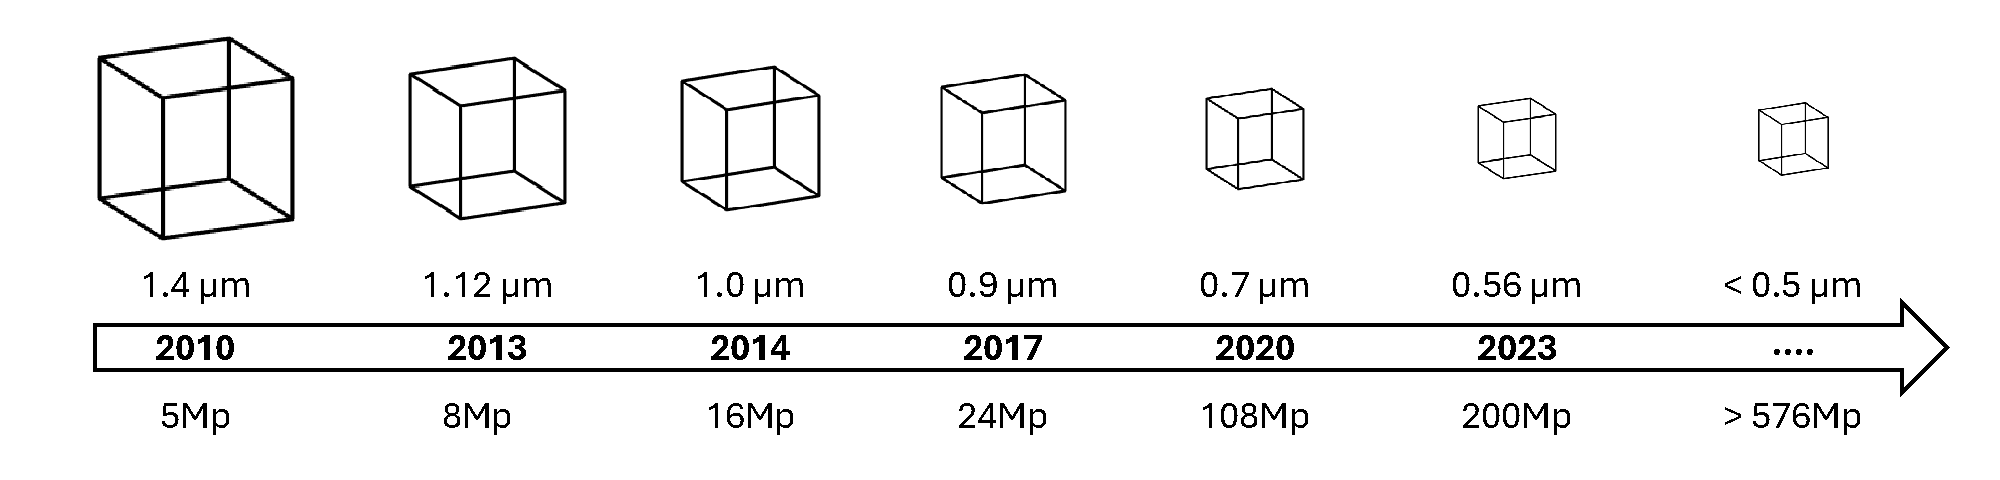
\includegraphics[width=.99\textwidth]{chapters/introduction/image/pixel_miniaturization.pdf}
  \caption [Pixel miniaturization roadmap.]{Scaling roadmap of the pixel pitch and resolution of CMOS image sensors. Adapted from: \cite{SookyoungRoh2025Dispersion-engineeredSensors}.}
  \label{fig:ch1:pixel_size}
\end{figure}

\subsection{Towards Ultra-High Resolution Imagers}

This rapid increase in resolution of CMOS image sensors has been primarily propelled by a reduction of the APS area, as shown in Figure~\ref{fig:ch1:pixel_size}. This has been enabled by multiple technological breakthroughs, including but not limited to, (i) the achievement of smaller nodes through advancements in lithography, (ii) the replacement of front-side illuminated (FSI) sensors (Figure~\ref{fig:ch1:backside_and_stacking}a) with back-side illuminated ones (BSI) (Figure~\ref{fig:ch1:backside_and_stacking}b), and (iii) the developments in stacked or 3D device integration (Figure~\ref{fig:ch1:backside_and_stacking}c-e). Even though the BSI configuration requires more complicated manufacturing with processing steps on both sides of the wafer, it effectively increases the sensor's quantum efficiency by removing the metallizations and dielectric layers between the microlens array and the photodiode \cite{Vici2020PerformanceConfiguration, Yaung2011HighShrinkage}. On the other hand, stacked device integration is an advanced packing approach that entails the vertical integration of pixel, logic, and analog-to-digital converter modules, effectively reducing the footprint of the CIS circuitry. This advancement was initially attributed to the through-silicon-via (TSV) technology and more recently to the Cu-Cu direct bonding technology \cite{Kagawa20193DSensors}. 

\begin{figure}[htbp]
    \centering
    % First plot
    \begin{subfigure}[t]{0.99\textwidth} % Adjust width as needed
        \centering
        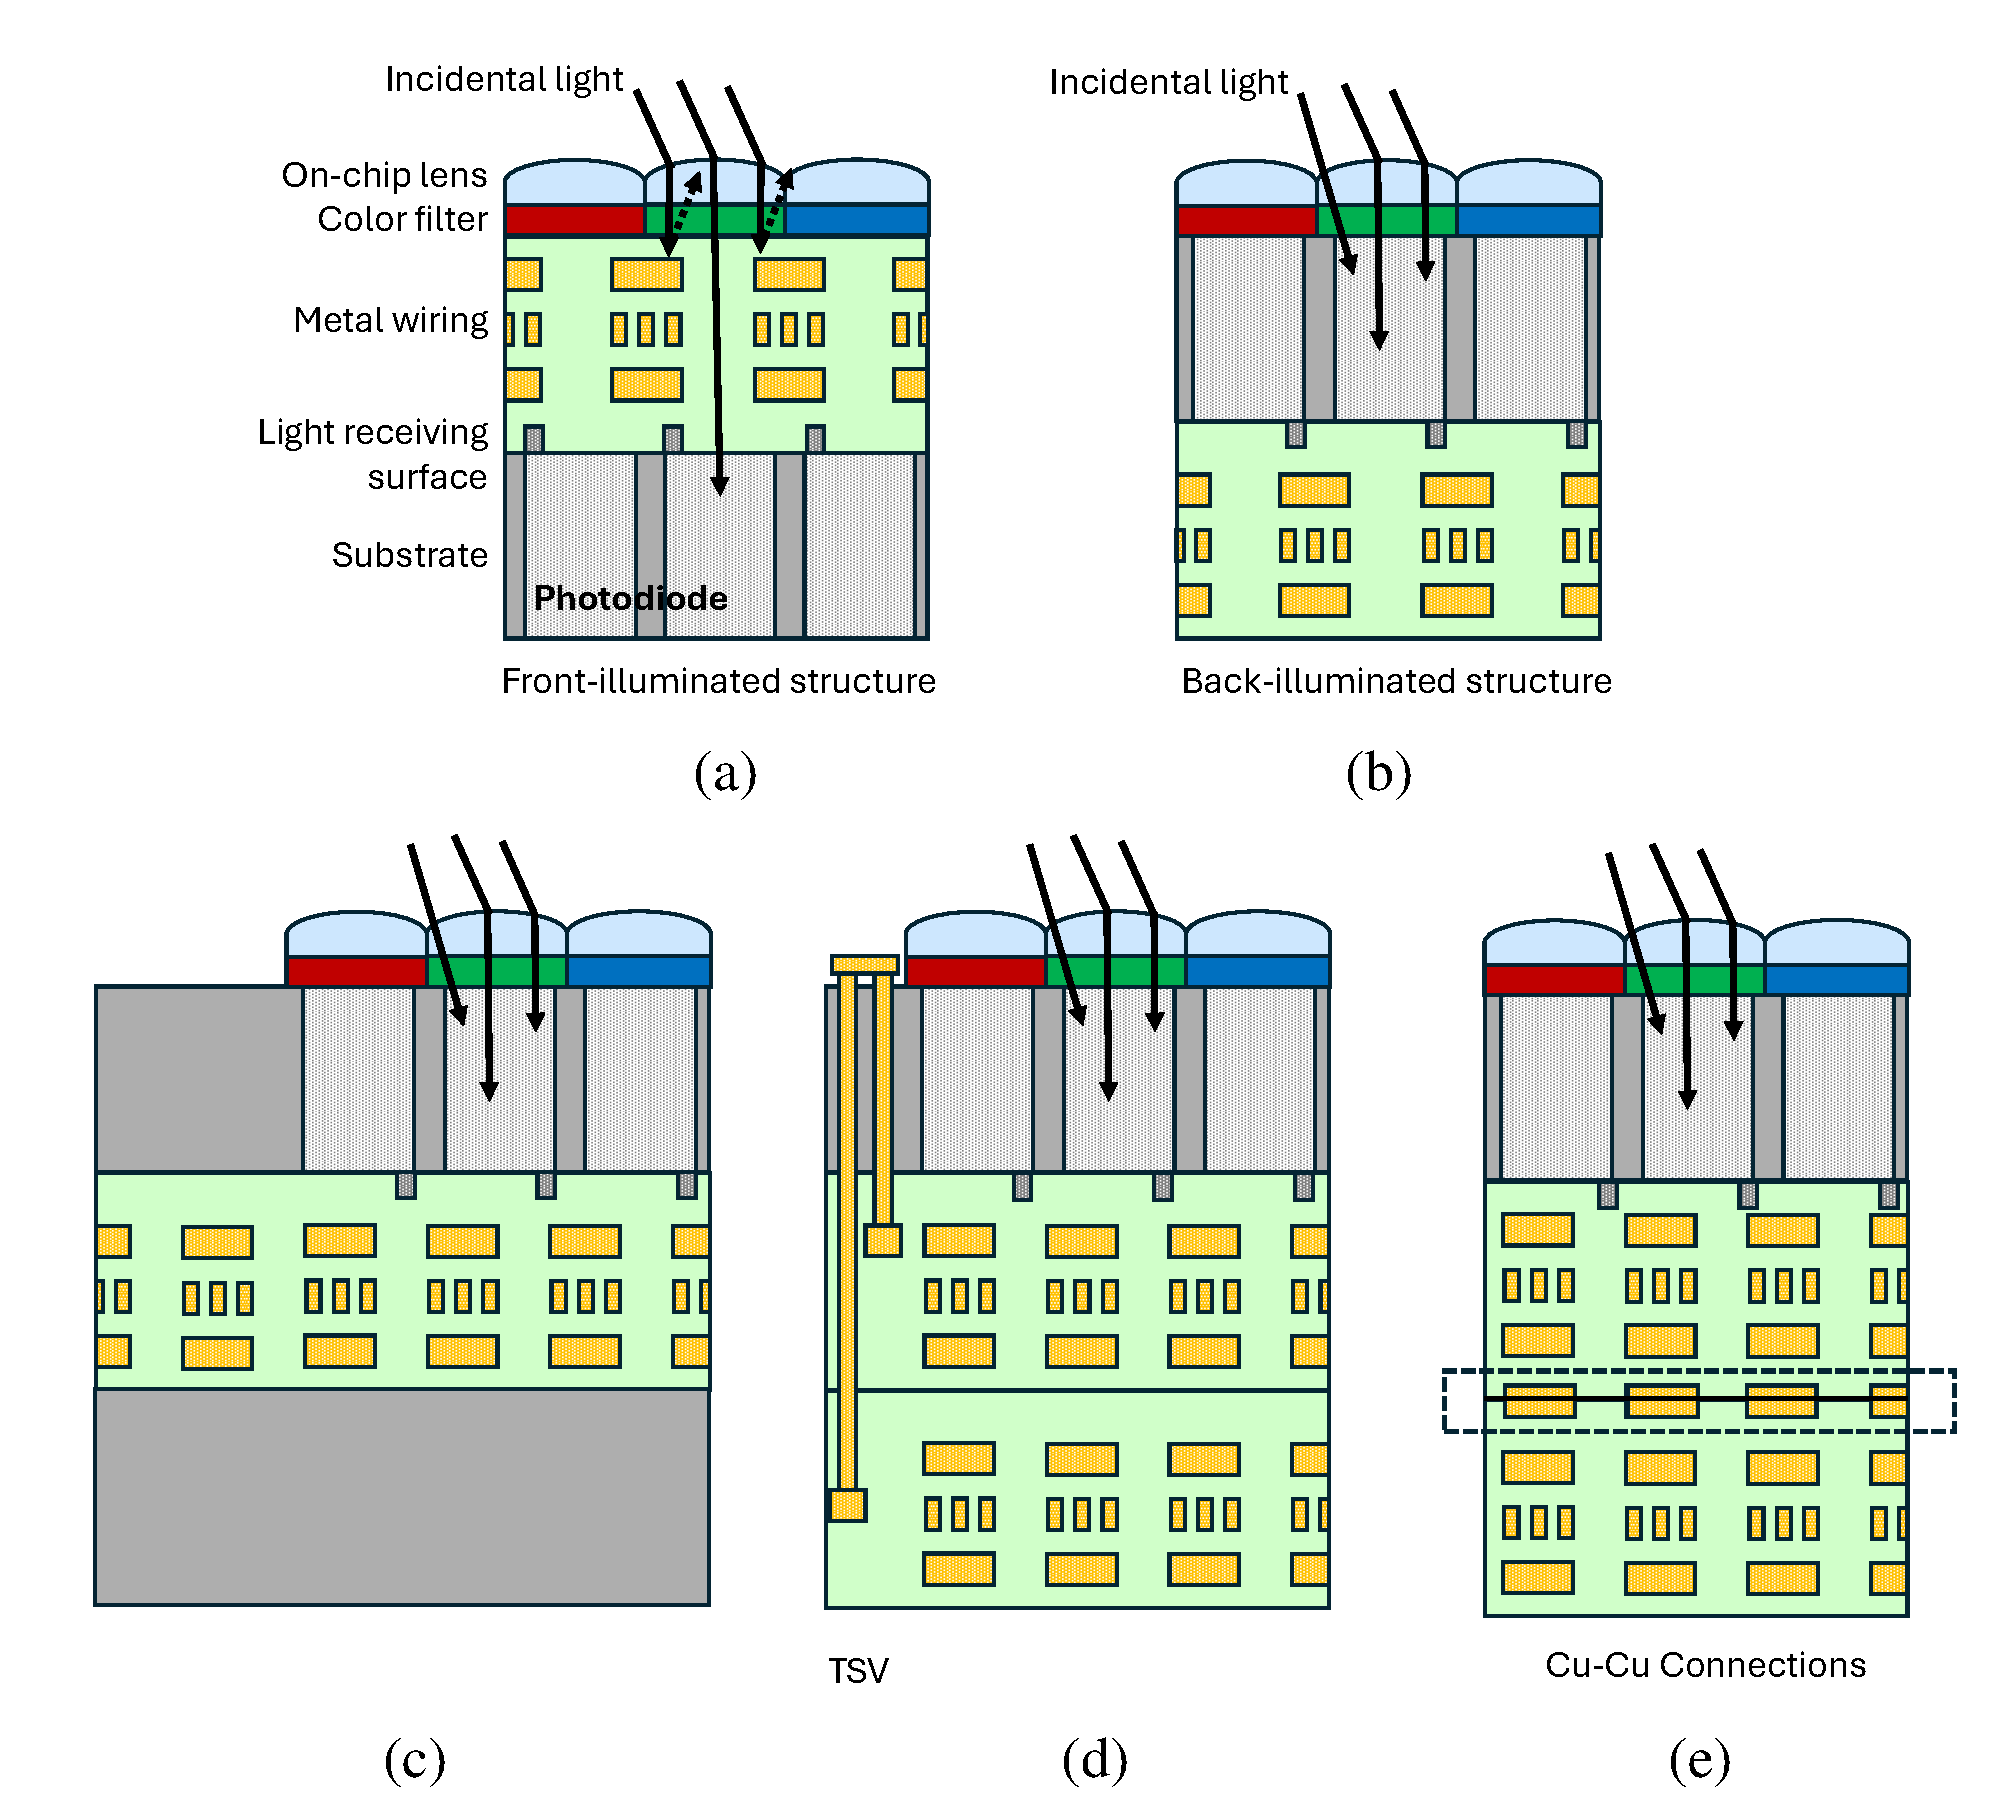
\includegraphics[width=\textwidth]{chapters/introduction/image/front_back_side_and_stacking.pdf} 
    \end{subfigure}
    % Caption for the whole figure
    \caption[Technological breakthroughs for the reduction of the APS area.]{Structure comparison for (a) front-side and (b) back-side illuminated CMOS image sensors. Adapted from \cite{SONY2008SonyNoise}. Structure comparison for (c) conventional and stacked CMOS image sensors, enabled by (d) TSV and (e) Cu-Cu direct bonding technology. Adapted from \cite{Kagawa20193DSensors}.}
    \label{fig:ch1:backside_and_stacking}
\end{figure}

Nevertheless, the miniaturization of APS pixels introduces new challenges, including increased pixel crosstalk and reduced light sensitivity. Crosstalk describes the leakage of photons and electrons between adjacent pixels, which in turn causes a degradation in image quality through blurring or desaturation \cite{Kim2022CrosstalkDeconvolution}. The first line of defense against crosstalk is the electrical and optical isolation of pixels using deep trench isolation (DTI), which relies on the reflection of oblique light within unit pixels. This process involves the etching of the area between two neighboring photodiodes, followed by its filling with materials including \ch{SiO_2}, poly-Si or tungsten \cite{Ahn2014AGate, Okawa2019ALevel, Kim2020ATechnology, Park20217.9Isolation}. A more recent, complimentary strategy focuses on the color filter array itself, employing a low refractive index grid that separates individual color filter units, minimizing diffraction and color crosstalk \cite{Han_Lin1.1umImprovement}.

Regardless of the various optimization techniques used to reduce crosstalk, the roadmap for pixel miniaturization sets a fundamental limit to the sensitivity of the image sensor, considering that the number of photons that can be captured by each pixel is proportional to the square of its size \cite{Kim2024FreeformSensors}. However, what initially seemed to be a dead end inspired the scientific community to pursue new directions and re-evaluate the necessity of CFAs for capturing color information, since it is well known that color filters, such as the Bayer pattern, absorb significant amount of the incoming light and hence reduce the signal to noise ratio (SNR). This realization has motivated efforts to replace CFAs with waveguides or metasurfaces, which, instead of absorbing unwanted photon wavelengths, redirect them to the appropriate photodiodes \cite{Nishiwaki2013EfficientSensors, Miyata2019High-SensitivityMetasurfaces, Kim2024FreeformSensors, Zou2022Pixel-levelMetasurfaces, Catrysse2022SubwavelengthEfficiency}. The fundamental difference between color filters and color routers and their impact on SNR is illustrated more clearly in Figure~\ref{fig:ch1:color_routing_concept}. Nonetheless, all of the reported color routing approaches are diffraction-based, meaning that the area of the APS cannot surpass the Abbe limit \cite{Shramkova2024HighSeparation}. 

\begin{figure}[ht!]
    \centering
    % First plot
    \begin{subfigure}[t]{0.6\textwidth} % Adjust width as needed
        \centering
        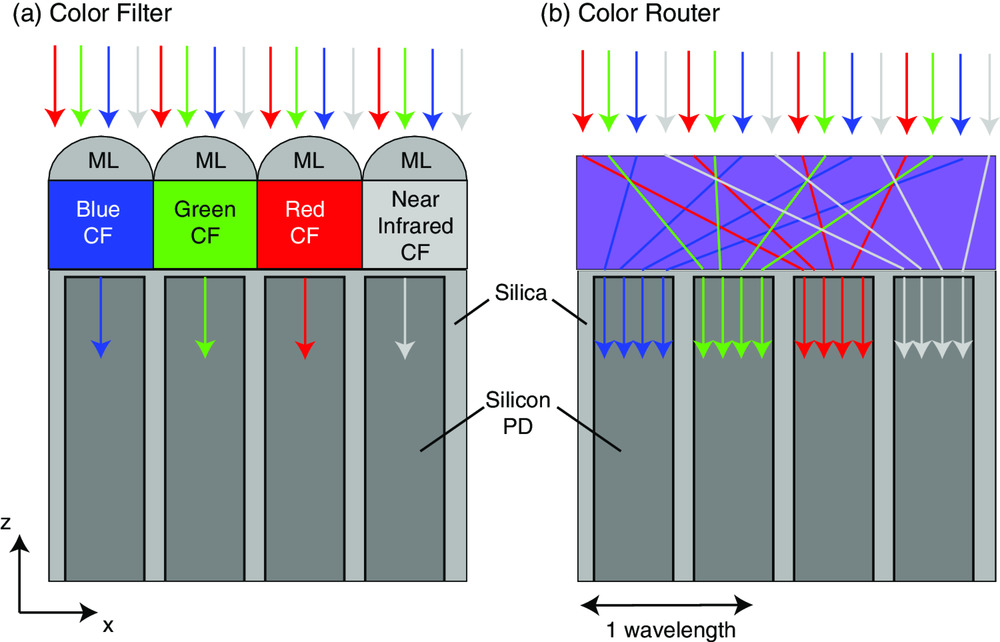
\includegraphics[width=\textwidth]{chapters/introduction/image/color_router.jpg} % Replace with your image
        \caption{}
        \label{fig:ch1:color_routing_concept}
    \end{subfigure}
    \hfill % Space between the two plots
    
    % Second plot
    \begin{subfigure}[t]{0.99\textwidth} % Adjust width as needed
        \centering
        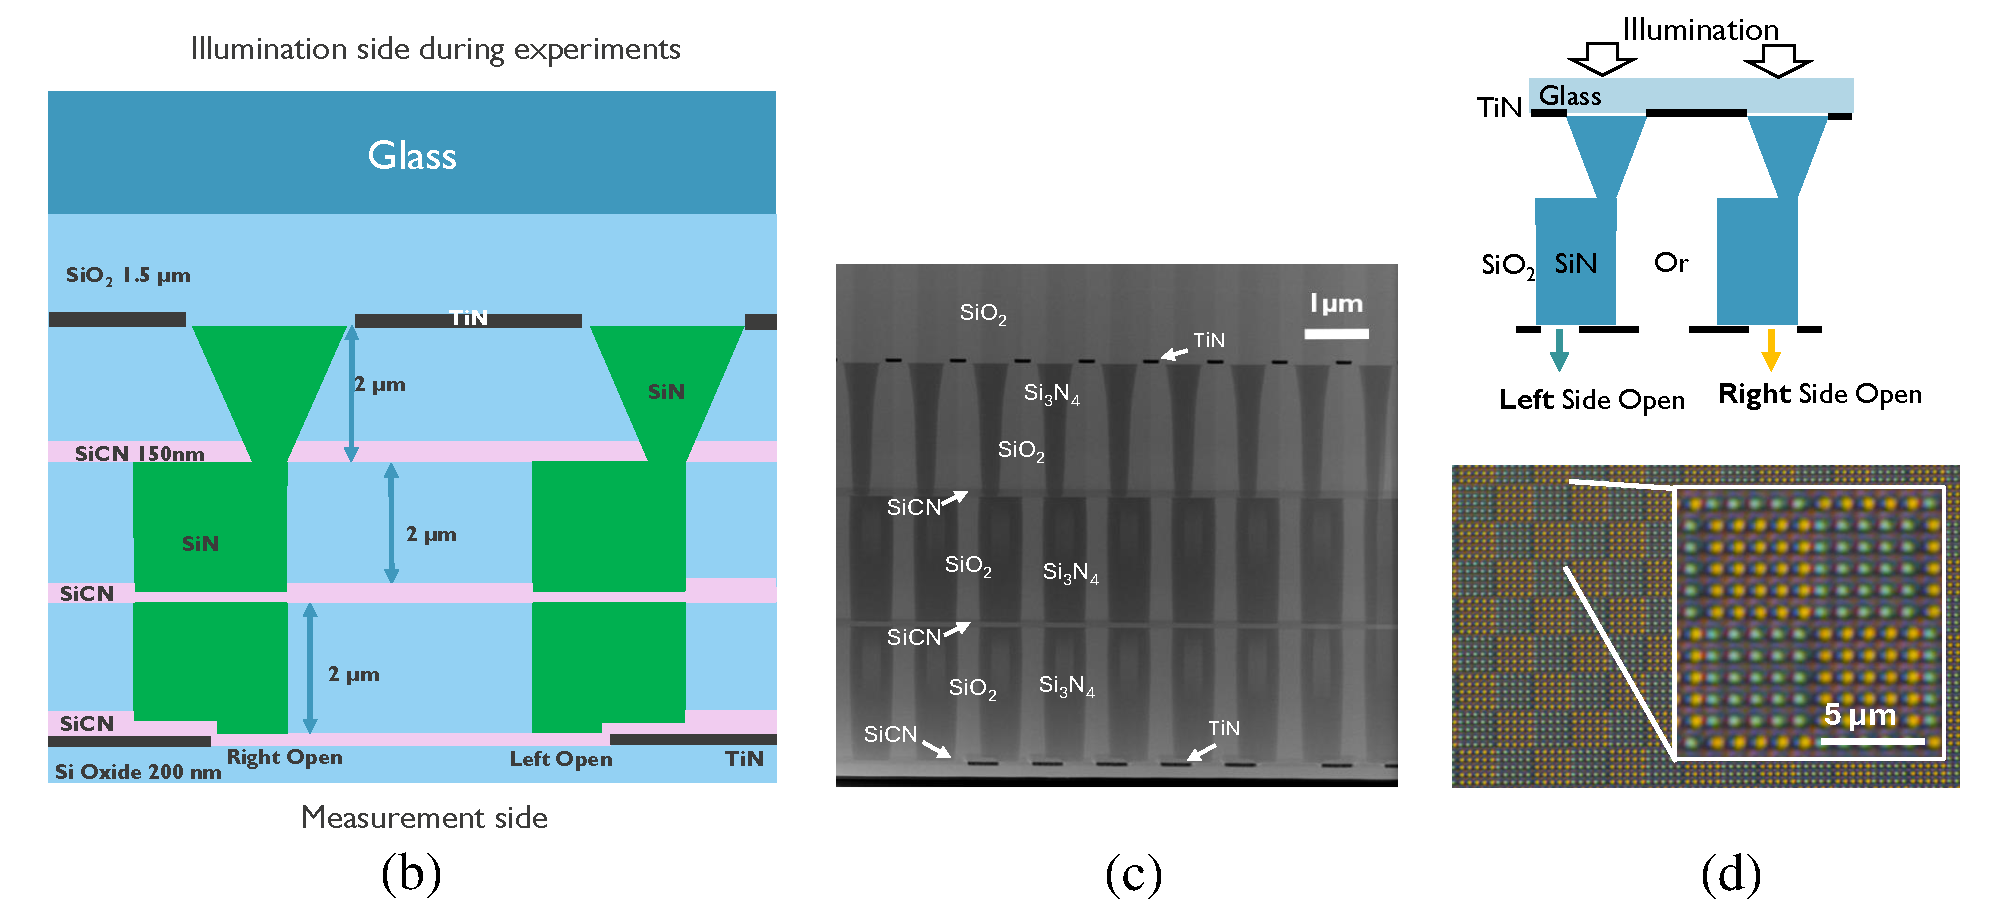
\includegraphics[width=\textwidth]{chapters/introduction/image/gigapixel_idea.pdf} % Replace with your image
    
    \end{subfigure}

    % Caption for the whole figure
    \caption[Introduction and implementation of color splitting technology.]{(a) Comparison of color sensing using traditional color filter (left) and emerging color router setups (right). Color routers replace the microlens (ML) and color filter (CF) array and direct incoming light, depending on its color, to the appropriate photodetector (PD). This way, nearly perfect efficiency for sub-wavelength pixels can be achieved. Reproduced from \cite{Zhao2021PerfectPixels}. (b) Conceptual and (c) fabricated cross-section of imec's color-splitting waveguide technology. (c) Visualization of the waveguides' characterization approach (top) and the corresponding  output, as captured from an RGB camera. Reproduced from \cite{Kang2017HighCsPbBr3}.}
    \label{fig:ch1:color_splitting}
\end{figure}

A major breakthrough in this regard was recently introduced by imec, which demonstrated that the Abbe-limited resolution can be surpassed with the use of multimode color-splitting waveguides that utilize the beating pattern of the interference between a symmetric and an asymmetric mode \cite{Kang2023Wafer-level-integratedSplitters}. Specifically, the color-splitter consists of a tapered waveguide that collects incoming light, squeezes it into single mode, and feeds it asymmetrically to a rectangular waveguide (Figure~\ref{fig:ch1:color_splitting}b). The symmetric and antisymmetric mode have different propagation speed in the rectangular waveguide, whose dimensions are carefully tuned such that the desired part of the visible spectrum is attained at the left or right side of its bottom opening. A cross-section of the fabricated \ch{Si_3N_4} waveguide in a \ch{SiO_2} matrix is shown in Figure~\ref{fig:ch1:color_splitting}c. For a demonstration of the color splitting efficiency of the waveguides, either the left or the right part of their exit was covered with a reflective TiN layer (Figure~\ref{fig:ch1:color_splitting}d - top) and the top of the waveguide was fed with white light illumination. The exit of the waveguide was monitored by an RGB camera, with results shown in (Figure~\ref{fig:ch1:color_splitting}d - bottom). A sharp separation between blue light and the rest of the spectrum was observed, while additional measurements revealed that the intensity ratio between the output and input light was more than 90\%, surpassing by far the efficiency of color filters. The inception of this technology opens the way for developing image sensors with pixel pitch as small as 0.2 $\mu m$ and is the main motivation for the work presented in the framework of this thesis. 


\subsection{Beyond Silicon Photodiodes}

Imec's color splitting waveguide technology has already demonstrated the possibility of leveraging more that 90\% of incoming light in the visible light range, which is far superior to color filters, and has opened the way for the continuation of pixel miniaturization to sub-wavelength dimensions. This advancement brings the crosstalk issue back into focus. 

Fundamentally, electrical and optical crosstalk is exacerbated by the weak absorption coefficient of the silicon photodetector (<$10^{4}$ $cm^{-1}$ for $\lambda$ > 500 nm) \cite{Herzinger1998EllipsometricInvestigation}, which requires a junction thickness close to 10 $\mu m$ to absorb 90\% of incoming visible light in a single pass. As long as the thickness of the absorbing layer remains constant and the pixel pitch continues to decrease, managing crosstalk will keep becoming increasingly more difficult \cite{Agranov2003CrosstalkSensor}. As a result, this observation provides the motivation to search for alternative materials with higher absorption efficiency in the visible spectrum that could potentially replace silicon and minimize the thickness of the photoconverting layer in a CMOS image sensor, effectively reducing crosstalk between neighboring pixels. 

For this reason, thin film photodetectors have emerged as a promising alternative in light sensing.  What defines the family of thin film materials is their high absorption coefficient which requires a physical thickness of only a few hundreds of nanometers to absorb all incident light. A common example of thin film photodetectors are bulk heterojunction organic photodiodes (OPDs), which have been intensely investigated over the past 20 years. OPDs rely on the mixing of donor (D) and acceptor (A) organic materials for the creation of precolating networks with large D/A area \cite{Scharber2013EfficiencyCells}. This solution was conceived to bypass the high exciton binding energy of organic semiconducting materials ($\sim$ 0.35 - 0.5 eV) and facilitate the exciton dissociation into free electron and hole pairs. Panasonic pioneered in the fabrication of high resolution organic image sensors without physical isolation between adjacent pixels \cite{Takase2015FirstFilm, Machida2018ASensitivity, Nishimura2016AnSensor, Nishimura2018AnCanceller}. Thanks to the low ratio of absorber thickness to pixel pitch, along with the implementation of electrical pixel isolation, the optical crosstalk in the demonstrated organic image sensors was significantly smaller compared to traditional Si image sensors. This development enables accurate color reproduction even in environments where conventional image sensors fail to reproduce original colors.

Nevertheless, the response speed of OPDs is inherently limited by the low mobility of the organic active material ($\sim$ 0.05 - 0.5 $cm^2V^{-1}s^{-1}$), limiting their potential for state of the art imaging applications, at least in the visible spectrum \cite{Nishimura2018AnCanceller}. Additionally, OPDs exhibit poor tolerance to high-temperature conditions, which further impairs their compatibility with standard semiconductor fabrication processes that involve high thermal budgets. As it will be further discussed in Section~\ref{sec:scope_and_aim}, this presents a critical limitation that must be taken into account when considering the fabrication of image sensors that employ the color-splitting waveguide technology. 


Over the past decade, metal halide perovskites have emerged as a promising alternative for thin-film photodetecting applications, propelled by their excellent optoelectronic properties and facile fabrication methods, which will be further expanded in the following section. Already, various research groups have demonstrated the integration of perovskite-based photodiodes (PePDs) with silicon \cite{Song2024HalideImager, Wang2024ASensor, Yen2016ALayer} or thin-film-transistor \cite{Deumel2021High-sensitivityPerovskites,vanBreemen2021APerovskites, Tsarev2025VerticallyPhotodetectors} readout integrated circuits (ROICs), proving their potential for fast and high-resolution imaging applications. These demonstrations utilize a monolithic integration approach, which means that the the ROIC is first fabricated using standard foundry processes, followed by the direct deposition of a thin-film photodetector layer on top, without a need for additional patterning steps. As a result, the resolution and pixel pitch of the image sensor is defined by the design  and properties of the ROIC. 


\section{Perovskite-Based Photodiodes (PePDs)}

\subsection{Properties of Perovskites}

\begin{figure}[htbp]
    \centering
    % First image (top)
    \begin{subfigure}[b]{\textwidth}
    \centering
        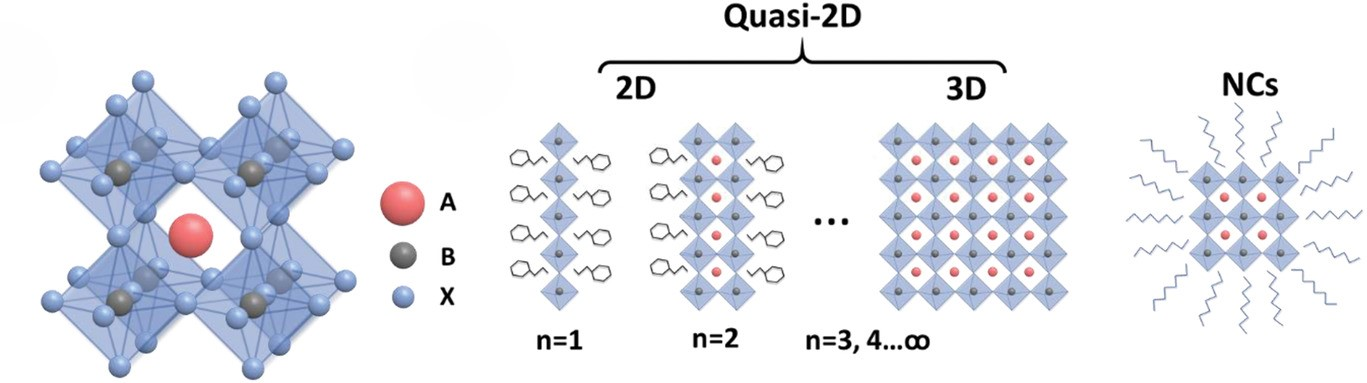
\includegraphics[width=0.85\linewidth]{chapters/introduction/image/perovskite_structure.jpg}
        \caption{}
        \label{fig:ch1:perovskite structure}
    \end{subfigure}

    \vspace{0.5cm}
    
    % Second image (bottom)
    \begin{subfigure}[b]{\textwidth}
    \centering
    %\hspace{-1.4cm}
        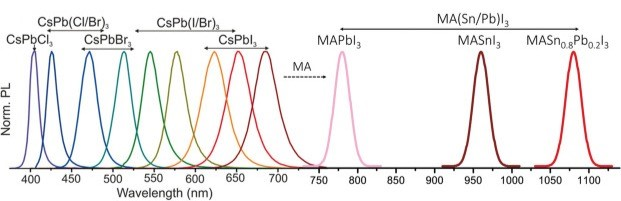
\includegraphics[width=0.85\linewidth]{chapters/introduction/image/bandgap_tunability.jpg}
        \caption{}
        \label{fig:ch1:bandgap_tunability}
    \end{subfigure}
    
    \caption[Perovskites' structure and bandgap tunability.]{(a) Perovskite crystal structure (left) and various morphologies (right). Reproduced from \cite{Lei2021MetalApplications}. (b) Photoluminescence emission wavelength for different composition of the perovskite active layer. Reproduced from \cite{Gholipour2020BandgapMaterials}.}
    \label{fig:ch1:perovskite_strucutre_bandgap}
\end{figure}

The term perovskite was introduced in 1839 to name the newly discovered, naturally occurring mineral of calcium titanate (\ch{CaTiO_3}). 170 years later, in 2009, metal halide perovskites were integrated for the first time in solar cell devices, inspiring their widespread use among groups around the world for the advancement of the third-generation photovoltaics \cite{Kojima2009OrganometalCells}. Since then, intensive scientific research has enabled single-junction perovskite cells to compete the power conversion efficiency (PCE) of the much more mature single-junction Si solar cells ($> 26\%$) \cite{Green2024Solar64}. Meanwhile, perovskite-Si tandem solar cells have demonstrated PCEs beyond the Shockley-Queisser limit ($>34\%$), establishing themselves as one of the most dominant candidates for next-generation solar technologies \cite{Hasan2024StabilityReview, Noman2024ATechnology}. This rapid growth of perovskite-based solar cell technology, from its inception to its commercial realization within 15 years, is attributed to both practical advantages and the exceptional optoelectronic properties of perovskites, as well. Practical advantages include, but are not limited to, low-cost production using abundant materials, and versatile fabrication through a wide variety of methods \cite{Fan2014Perovskite-basedCells}. On the other hand, some remarkable optoelectronic properties of perovskites are their tunable and direct bandgap \cite{Gholipour2020BandgapMaterials}, high absorption coefficient (> $10^4$ $cm^{-1}$) \cite{Park2015PerovskiteTechnology}, low exciton binding energy (<0.05 eV) \cite{Lin2015Electro-opticsCells}, defect tolerance \cite{Kumar2021RoleApplications}, and high carrier mobility (1-100 $cm^2V^{-1}s^{-1}$) \cite{Herz2017Charge-CarrierLimits}. 


Metal halide perovskites can be divided into three groups, each of which has distinct properties: (i) three-dimensional (3D), (ii) two-dimensional (2D) and (iii) zero-dimensional (0D) perovskites. Structures that incorporate both 2D and 3D perovskite characteristics are known as quasi-2D perovskites (Figure~\ref{fig:ch1:perovskite structure}). 3D perovskites can be generally described by the \ch{ABX_3} formula, where A is a 12-fold-coordinated monovalent cation such as methylammonium (\ch{MA^+}), formamidinium (\ch{FA^+}), or cesium (\ch{Cs^+}), B is a 6-fold-coordinated inorganic divalent inorganic cation such as lead (\ch{Pb^{2+}}) and tin (\ch{Sb^{2+}}), while X is a strongly electronegative monovalent halide anion (\ch{I^-}, \ch{Br^-}, and \ch{Cl^-}). As a result, mixed compositions can be pursued for each lattice site, enabling the tuning of the perovskite's bandgap across a wide range of energies (spanning from near ultraviolet (UV) to near infrared (NIR)), depending on the desired application (Figure~\ref{fig:ch1:bandgap_tunability}).

\subsection{From Solar Cells to Photodetectors}

The rapid advancements of perovskite-based solar cells (PeSCs) sparked interest for their use in alternative optoelectronic applications, including photodetectors, light-emitting diodes (LEDs), and lasers. While solar cells operate without external bias, photodetectors typically operate in the reverse bias regime to promote faster carrier extraction, while lasers and LEDs operate in the forward bias regime to promote radiative recombination. While the diode structure is similar for all applications, the different operational regimes introduce distinct challenges for each use. Nevertheless, the operation of solar cells and photodiodes is more closely related, as they both depend on the efficient extraction of the photo-generated carriers. This process relies on the photovoltaic effect, during which the incoming light is absorbed by the active material, as long as its energy is equal or larger than the bandgap, leading to the generation of electron-hole pairs (or excitons). Under the effect of the built-in potential, which may be complimented by an additional field through external biasing, the charge carriers are extracted and collected at the respective contacts as photocurrent. 

The solar cell structure, as well as the photodetectors that are developed in the framework of this thesis rely on the on the photodiode structure (Figure~\ref{fig:ch2:types_of_detector}a), a vertical structure where the active layer is sandwiched between two charge transport layers, commonly referred to as the electron transport layer (ETL) and the hole transport layer (HTL). The role of these layers is typically twofold: (i) they promote the efficient extraction of the photo-generated carriers, and (ii) they block the injection of the opposite carrier from the electrode under the effect of reverse bias. The latter condition is only true for occasions where wide-bandgap transport layers are used. When developing the photodiode stack on top of a glass substrate, the architecture can be further distinguished in p-i-n and n-i-p, depending on the whether the perovskite is processed is processed on top of the HTL or ETL, respectively. 

The photodiode is not the only structure that is used for photo-detecting applications. Two additional types of photodetectors include the two-terminal photoconductors and the three-terminal phototransistors (Figure~\ref{fig:ch2:types_of_detector}b and Figure~\ref{fig:ch2:types_of_detector}c, respectively), which have both a lateral geometry. Both architectures rely on a gain mechanism, which leads to a slower response time. At the same time, the relatively large spacing between the electrodes (> 10 $\mu m)$. not only requires a higher driving voltage but is also unsuitable for integration with readout circuits that have a significantly smaller pixel pitch (below 5 $\mu m)$.

\begin{figure}[htbp]
  \centering
  \medskip
  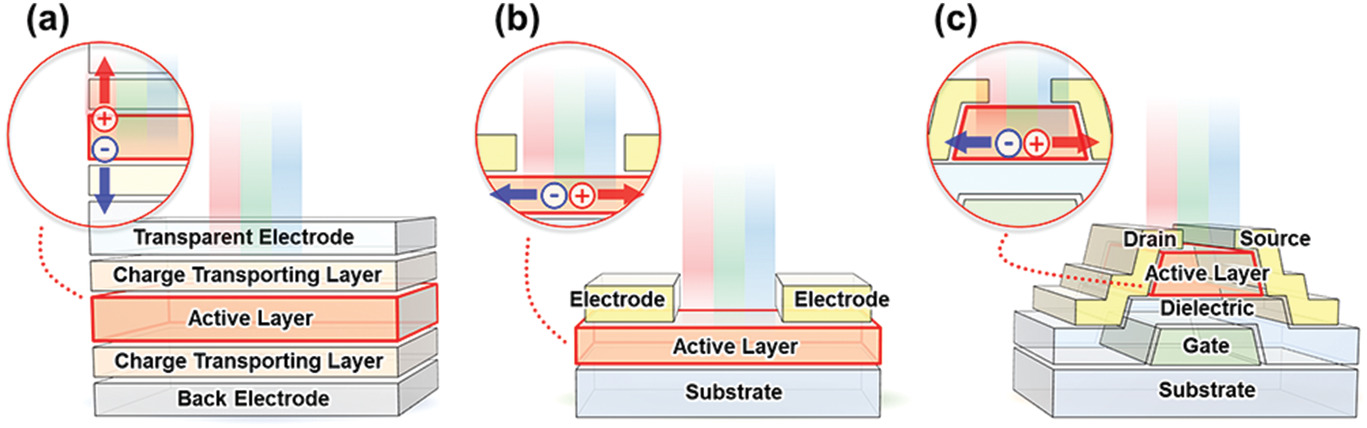
\includegraphics[width=.9\textwidth]{chapters/introduction/image/types_of_detector.jpg}
  \caption[Comparison of photodetector structures.]{Schematic illustration of different types of photodetectors depending on device structure, including (a) photodiodes, (b) photoconductors, and (c) phototransistors. Reproduced from \cite{Yoo2021ADirections}.}
  \label{fig:ch2:types_of_detector}
\end{figure}

\subsection{Scalable and High-Temperature PePDs} \label{ch1:scalable_high_temp}


The vast majority of studies on perovskite-based optoelectronic devices rely on the use of solution processed methods, and specifically spin-coating. This is not surprising, considering that spin-coating is a technique that is simple, easily accessible, and has low cost. These characteristics make it highly suitable for rapid prototyping and exploration of various material combination that can promote efficiency or stability. For example, during solution preparation it is common to include various additives that in turn can help modulate morphology, optimize energy level-alignment or eliminate hysteresis \cite{Liu2020ACells}. However, cell fabrication through spin-coating is not transferable to industry, due to limitations in throughput and large-area deposition. For example, a commonly used technique, anti-solvent processing, has been shown to be challenging to scale-up \cite{Saki2021Solution-processedCells}.

\begin{figure}[htbp]
  \centering
  \medskip
  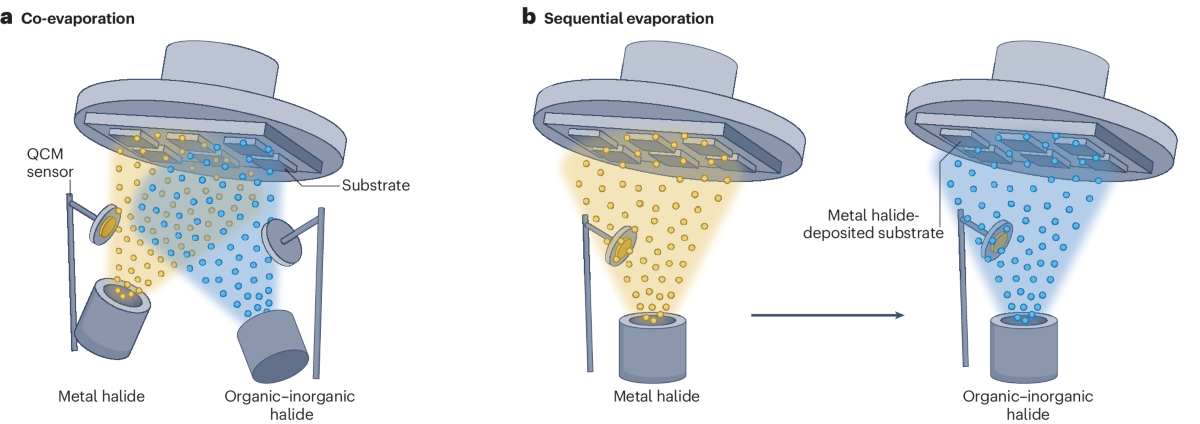
\includegraphics[width=.99\textwidth]{chapters/introduction/image/types_of_evaporation.png}
  \caption[Comparison of vacuum deposition approaches.]{Schematic illustration of different types of vacuum deposition methods, including (a) co-evaporation, and (b) sequential evaporation. Reproduced from \cite{Han2025PerovskiteCells}.}
  \label{fig:ch2:types_of_evaporation}
\end{figure}

Significant efforts have been made to explore alternative fabrication techniques that enable the scalable deposition of perovskite-based devices. Such methods involve solution-processed approaches (such as inkjet printing \cite{Zhang2023ProgressApplications} and spray coating \cite{Bishop2020DevelopmentCells}) or vacuum-processed ones (such as chemical vapor deposition \cite{Magubane2023SequentialTransport} or thermal evaporation \cite{Wang2024ThermallyBeyond}). Among those, thermal evaporation is the most mature one, and as of 2020 it enabled the fabrication of 21 $cm^2$ solar cell mini modules with the superior efficiency of 18.13\% \cite{Vaynzof2020TheProcessing, Li2020HighlyMini-modules}. Besides scalability, thermal evaporation offers the advantage of not necessarily requiring a post-deposition thermal annealing step, rendering highly attractive for applications that require the use of flexible substrates \cite{Becker2019LowExperimentation}. On top of that, it avoids the use of toxic solvents, allows for precise control of the deposited thickness, and prevents the risk of damaging the underlying layers in tandem structures \cite{Zhang2020TowardCells, Forgacs2017EfficientCells}

Evaporation of perovskite thin films can be categorized into co-evaporation and sequential evaporation, as shown in Figure~\ref{fig:ch2:types_of_evaporation}a and Figure~\ref{fig:ch2:types_of_evaporation}b, respectively. Co-evaporation entails the simultaneous evaporation of the necessary precursors, rendering the careful monitoring and maintenance of evaporation rates ratio as highly crucial \cite{Frolova2017HighlyPbI2,Abzieher2021FromCells}. On the other hand, in sequential evaporation each precursor is deposited individually, rendering the thickness of each layer as the defining parameter for the perovskite's stoichiometry \cite{Liu2019SequentiallyCells, Burschka2013SequentialCells, Li2022SequentialEfficiency}. Unlike co-evaporation, a post-deposition thermal annealing step is essential for sequentially deposited films to facilitate the reaction and intermixing of precursors, enabling the formation of the perovskite film. A third option for the evaporation of perovskite thin film, which is not illustrated, is the single-source evaporation \cite{Zheng2019SingleApplications, Soto-Montero2024Single-SourceCells, Li2020FabricationEvaporation}. This approach requires an initial synthesis of the perovskite via powder mixing or crystal growth. Followingly, the powder mixture or the pulverized crystals are loaded in a single substrate from which they are evaporated. 


Despite the advantages of using thermal evaporation for the deposition of perovskite-based optoelectronic devices, several limitations still exist. For instance, the high vacuum pressure and low sticking coefficient of \ch{MA^+} renders its evaporation rather complicated \cite{Kim2020DepositionPerovskite}. At the same time, the inclusion of additives, which is crucial for improving the performance/stability of solution-processed films, is not compatible with evaporation. Lastly, evaporated perovskite films tend to have significantly smaller grain sizes, which may compromise their stability against moisture or limit device performance due to their higher defect density \cite{Vaynzof2020TheProcessing, Wang2017ScalingFilms}.


Besides the use of spin-coating as the fabrication technique, research around perovskite optoelectronic devices is mainly focused on the use of hybrid organic-inorganic perovskites, where the A-site cation is a mixture of \ch{MA^+}, \ch{FA^+}, and/or \ch{Cs^+}, leading to optimal performances \cite{Zhang2021All-inorganicCells}. However, perovskites that contain organic molecules are more sensitive to thermal degradation. For instance, it was shown that methylammonium-based perovskites decompose into methylamine, hydrogen iodide, and lead iodide for temperatures beyond 100 \degree C. This limitation renders hybrid organic-inorganic perovskites unsuitable for applications with high thermal budget, which may be imposed by intrinsic (triggering of self-heating mechanisms through resistive loses) or extrinsic factors (high ambient temperature, high temperature post processing) \cite{Handa2019LargePerovskite, Dong2023GrowthFilm, Li2022StructureTemperatures}. 

\begin{figure}[htbp]
    \centering
    % First plot
    \begin{subfigure}[t]{0.56\textwidth} % Adjust width as needed
        \centering
        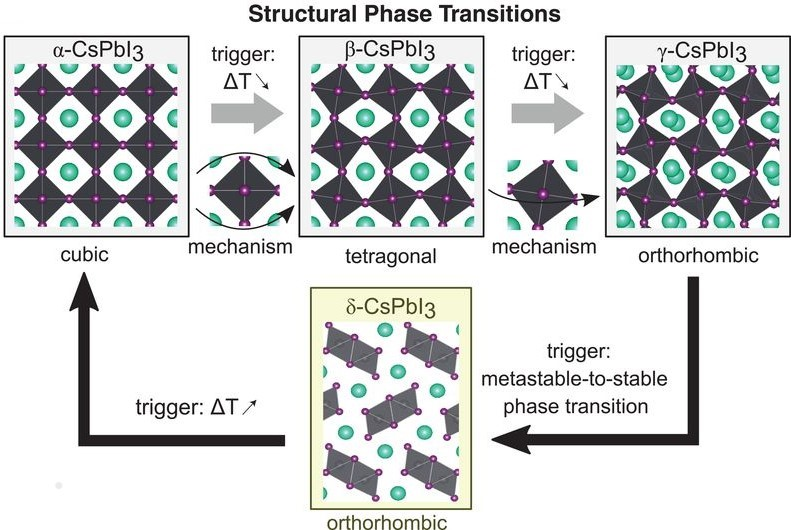
\includegraphics[width=\textwidth]{chapters/introduction/image/perovskite_phases.jpeg} % Replace with your image
        \caption{}
        \label{fig:ch2:perovskite_phases}
    \end{subfigure}
    \hfill % Space between the two plots
    % Second plot
    \begin{subfigure}[t]{0.39\textwidth} % Adjust width as needed
        \centering
        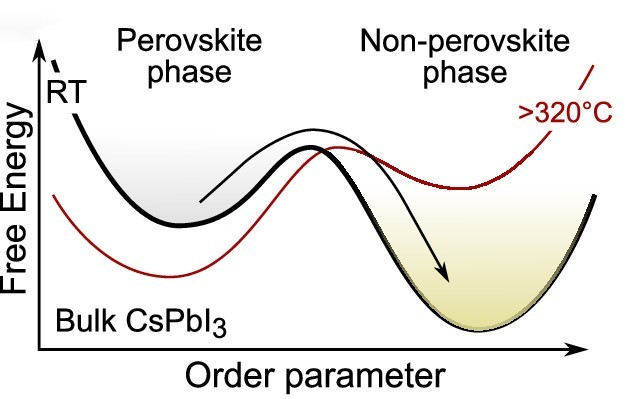
\includegraphics[width=\textwidth]{chapters/introduction/image/perovskite_free_energy.jpeg} % Replace with your image
        \caption{}
        \label{fig:ch2:perovskite_free_energy}
    \end{subfigure}

    % Caption for the whole figure
    \caption[Phase transitions and phase stability for the \ch{CsPbI_3} composition.]{(a) Phase transitions for the \ch{CsPbI_3} perovskite and their respective crystal structure. Reproduced from \cite{Steele2019ThermalFilms}. (b) Illustration of energy diagram for the competing perovskite (black) and non-perovskite (yellow) phases at room temperature and above 320 \degree C. At room temperature (black scheme) the perovskite phase is metastable because the non-perovskite phase has the lowest free energy. Reproduced from \cite{Steele2021TrojansPerovskite}.}
    \label{fig:ch2:phases_and_free_energy}
\end{figure}

Under these circumstances, all-inorganic perovskites, in the \ch{CsPbI_{x}Br_{3-x}} ($0 \le x \le 3$) family become an attractive solution, since they have been proven to withstand temperatures beyond 250 \degree C \cite{Dong2021High-TemperatureCells}. The two endmembers of this composition are \ch{CsPbI_3} and \ch{CsPbBr_3}. The latter has a bandgap close to 2.3 eV ($\sim$ 540 nm), which is unsuitable for visible light detection, considering that it completely excludes the red part of the spectrum \cite{Tong2020RecentCells}. On the other hand, \ch{CsPbI_3} has a reported bandgap in the range of 1.7 eV, allowing for the detection of the complete visible light spectrum \cite{Zhao2018ThermodynamicallyPhotovoltaics}. However, \ch{CsPbI_3} exists in several phases, and the photoactive (black) phases are only stable in elevated temperatures. In room temperature, a yellow, non-perovskite phase ($\delta-$ \ch{CsPbI_3}) with significantly larger bandgap (~2.8 eV) is the thermodynamically preferred one, rendering it unsuitable for any kind of optoelectronic applications (Figure~\ref{fig:ch2:perovskite_phases}) \cite{Cho2021Long-termNetwork, Burwig2018CrystalFilms, Steele2022AnFilms}. The black phase consists of the $\gamma-$ (orthorhombic), $\beta-$ (tetragonal), and $\alpha-$ (cubic) phase, which are similar in structure and properties and emerge beyond 320 \degree C (Figure~\ref{fig:ch2:perovskite_free_energy}). It is possible to kinetically trap the black phase at room temperature through rapid cooling, however the yellow phase re-emerges almost instantaneously when the perovskite film is exposed to ambient moisture \cite{Steele2019ThermalFilms}. 

To develop a better understanding of the stability or perovskite phase and ways to enhance it, it is important to introduce a few new parameters, namely the tolerance factor (t), the octahedral factor ($\mu$), and the atomic packing fraction ($\eta$). The Goldschmidt tolerance factor, defined as:
\begin{equation}
    t = \frac{r_A + r_X}{\sqrt{2}(r_B + r_X)},
    \label{eq:tolerance_factor}
\end{equation} 

where $r_A$, $r_B$, and $r_X$ are the ionic radius of the A, B, and X sites, respectively \cite{Goldschmidt1926DieKrystallochemie}. A perovskite can be formed for $0.8 < t < 1.0$, where $t = 1$ represents an ideal cubic perovskite. The octahedral factor represents the ratio between the radii of the B-site cation and the X-site anion ($\mu = r_B/r_X$), while the atomic packing factor (APF) describes the fraction of a crystal structure's total volume that is occupied by its constituent atoms. Using this parameters, Sun et al. introduced a stability descriptor ($(\mu + t)^2$), that can predict the relative stability between two perovskites and is visualized in Figure~\ref{fig:ch2:perovskite_stable_region} \cite{Sun2017ThermodynamicPerovskites}. Taking the computational error into account, it can be seen that the \ch{CsPbI_3} composition is on the borderline between the stable and non-stable region, explaining its metastable behavior at room temperature.  

\begin{figure}[htbp]
  \centering
  \medskip
  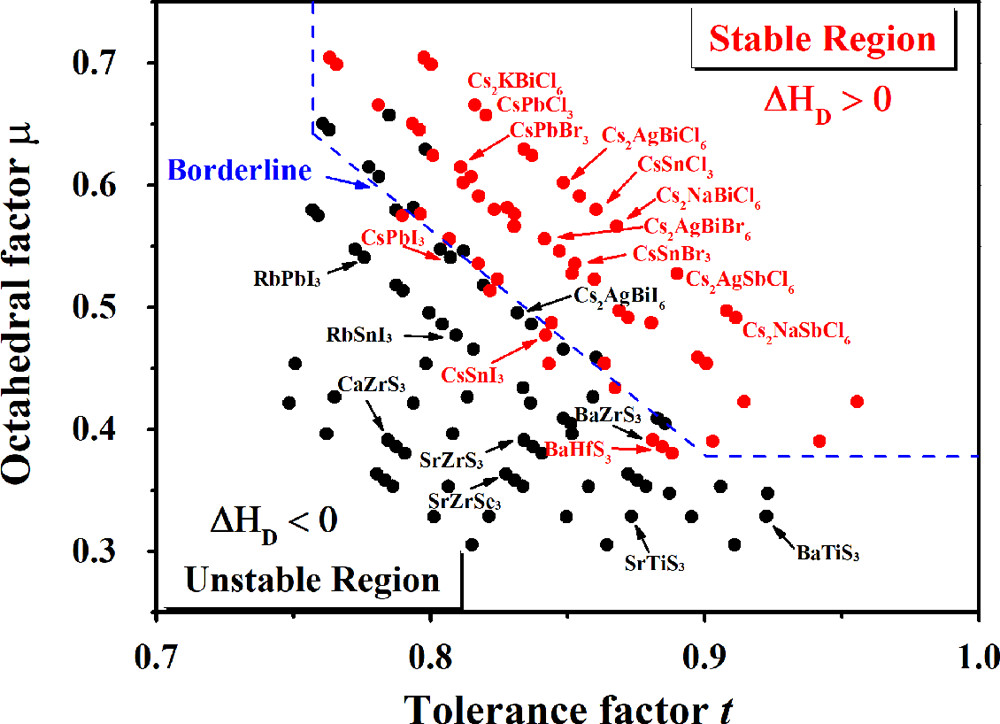
\includegraphics[width=.67\textwidth]{chapters/introduction/image/perovskite_stability.jpeg}
  \caption[Stability of various perovskite compositions as a function of their octahedral and tolerance factors.]{Map of decomposition energy ($\Delta H_D$) for various perovskite compounds, which is defined by their octahedral and tolerance factor. The blue dashed line separates the stable (red dots - $\Delta H_D>0$) from the non-stable (black dots - $\Delta H_D<0$) region. Reproduced from \cite{Sun2017ThermodynamicPerovskites}.}
  \label{fig:ch2:perovskite_stable_region}
\end{figure}

Several strategies have been explored to enhance the stability of \ch{CsPbI_3} in ambient conditions, including component engineering, additive engineering, dimensionality reduction engineering and phase mixing engineering \cite{Lei2024StabilityPerovskites, Jin2024PhaseDevices}. Component engineering, achieved through the partial replacement of the A-, B-, or X-sites, enables composition shifts toward the stable region of Figure~\ref{fig:ch2:perovskite_stable_region}, while maintaining compatibility with thermal evaporation and avoiding the use of organic compounds. Such effect can be achieved by partially replacing \ch{I^-} with \ch{Br^-}. The latter has a smaller ionic radius, effectively increasing the crystal's tolerance factor. However, a trade-off between stability and bandgap suitability arises, considering that the engineered composition moves closer to \ch{CsPbBr_3}, which is transparent for the red part of the visible spectrum. A reasonable compromise between phase stability and visible light detection is reached with \ch{CsPbI_2Br}, with a bandgap in the range of $\sim$ 1.95 eV (635 nm) \cite{Nasstrom2020DependenceExperimentation}. Such a composition can be easily achieved via the co-evaporation of CsBr and \ch{PbI_2} powders in a one-to-one molar ratio. A variety of reports have employed the \ch{CsPbI_2Br} composition, either through solution processing \cite{Roy2025All-inorganicLayers, Zhang2019HighCells,Dong2021High-TemperatureCells,Zhang2021ModificationEfficiency,Wang2020HighlyBase,Zheng2021ImprovedCells,Mariotti2018StabilityDevices,Mali2019Hot-Air-AssistedCells}  or vacuum deposition \cite{Lin2019EfficientDeposition,Chen2017All-Vacuum-Deposited11,Igual-Munoz2020Room-TemperaturePrecursors, Ma2017TheCells, Lai2022All-Vacuum-DepositedCm-3}, for the fabrication of solar cells and photodiodes. However, even reports investigating the use of vacuum deposited inorganic perovskites are routinely using solution processed and/or organic transport layers, a practice that counterbalances the advantages of the selected active layer. 


\section{Scope and Aim of This Thesis} \label{sec:scope_and_aim}

The scope of this thesis is defined by the emergence of color-splitting waveguides and the identification of perovskite thin films as a promising active layer for ultra-high-resolution CMOS imagers with minimized pixel crosstalk. The conceptual design of such an imager is illustrated in Figure~\ref{fig:ch1:scope}a, while Figure~\ref{fig:ch1:scope}b presents the proposed process flow for its fabrication. In the framework of this thesis, the focus is directed to the development of a perovskite-based photodetector that can be monolithically integrated on top of a silicon readout integrated circuit (ROIC) and satisfies the requirements of high scalability and temperature tolerance. The condition of high-temperature tolerance (> 250 \degree C) is imposed by the 4th step in the proposed process flow, that requires the direct bonding of the waveguide matrix and the underlying CMOS image sensor using silicon oxide (\ch{SiO_2}) or silicon-carbon-nitride (SiCN) bonding. Specifically, a post-bonding thermal annealing step at temperatures beyond 250 \degree C is necessary for the attainment of a high bond strength with minimal voids and defects. Taking into account the additional requirements for scalability and compatibility with CMOS processing, the use of thermally evaporated inorganic metal halide perovskites (\ch{CsPbI_2Br}), integrated into vacuum-deposited, all-inorganic photodiodes, emerges as a promising approach that meets the aforementioned prerequisites.


\begin{figure}[htbp]
    \centering
    % First plot
    \begin{subfigure}[t]{0.99\textwidth} % Adjust width as needed
        \centering
        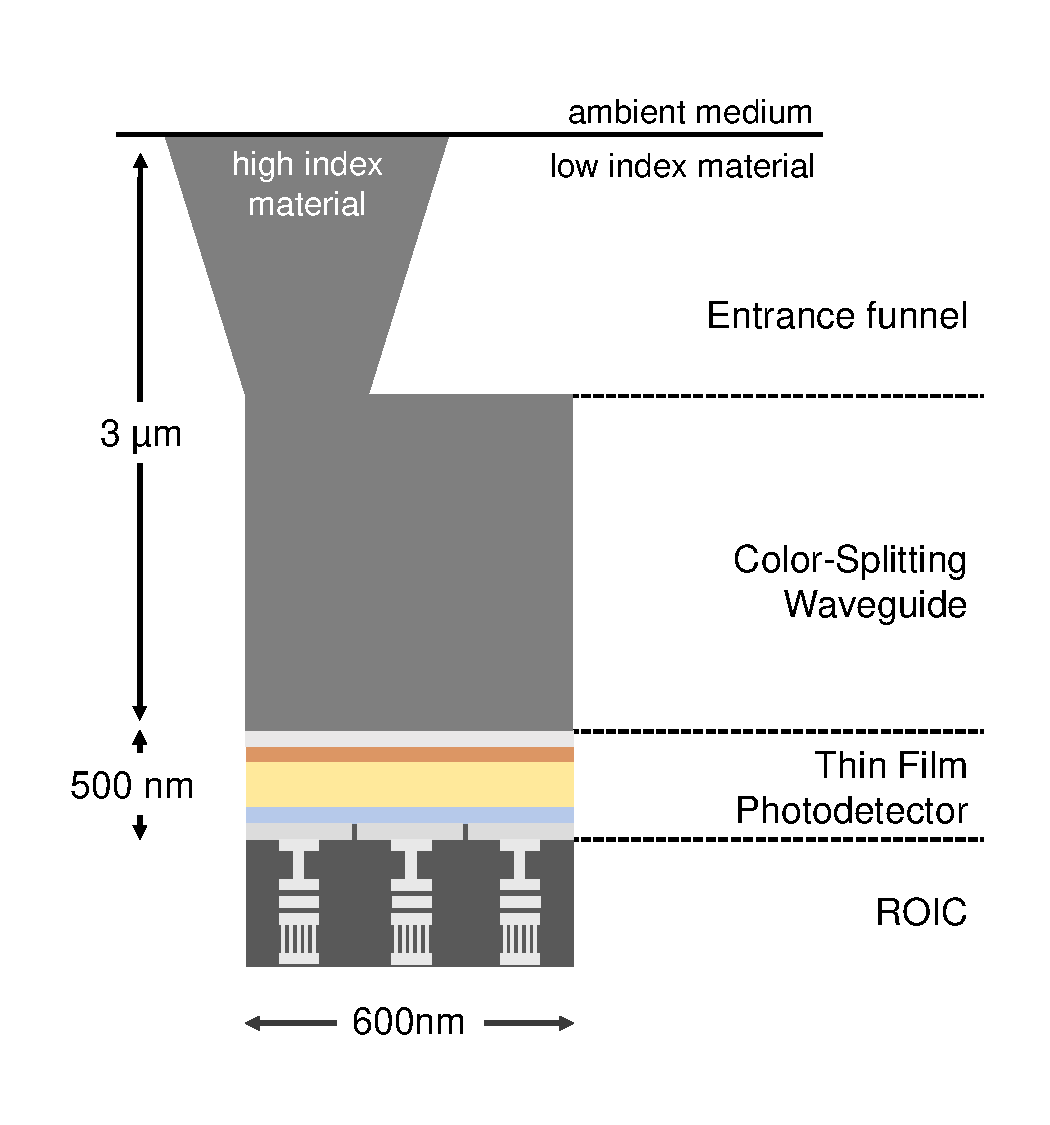
\includegraphics[width=\textwidth]{chapters/introduction/image/waveguide_pepd.pdf} % Replace with your image
    \end{subfigure}

    % Caption for the whole figure
    \caption[Conceptualization and proposed fabrication steps of image sensors, utilizing color-splitting waveguide technology.]{(a) Conceptual design of a PePD-integrated CMOS imager using color-splitting waveguide technology for color sensing and (b) proposed process flow for its fabrication.}
    \label{fig:ch1:scope}
\end{figure}



\begin{figure}[htbp]
    \centering
    % First plot
    \begin{subfigure}[t]{0.6\textwidth} % Adjust width as needed
        \centering
        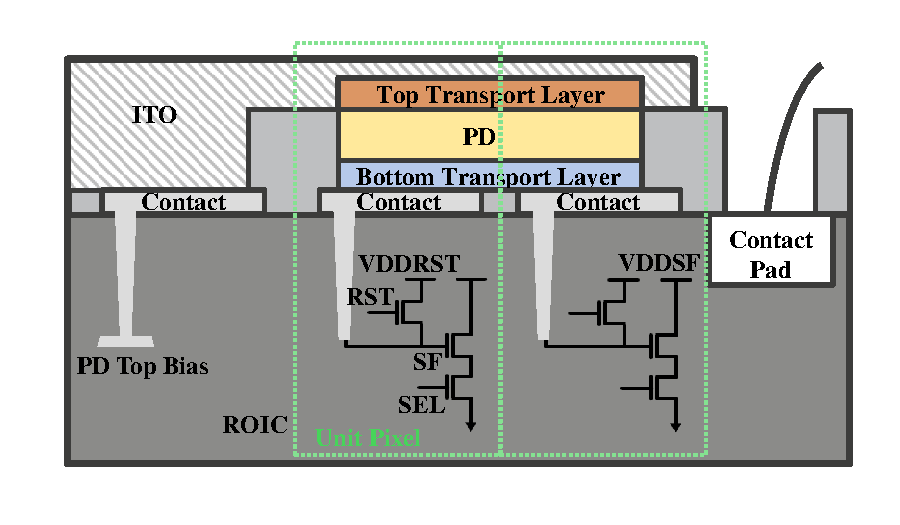
\includegraphics[width=\textwidth]{chapters/introduction/image/imager_cross_section.pdf} % Replace with your image
        \caption{}
        \label{}
    \end{subfigure}
    \hfill % Space between the two plots
    % Second plot
    \begin{subfigure}[t]{0.99\textwidth} % Adjust width as needed
        \centering
        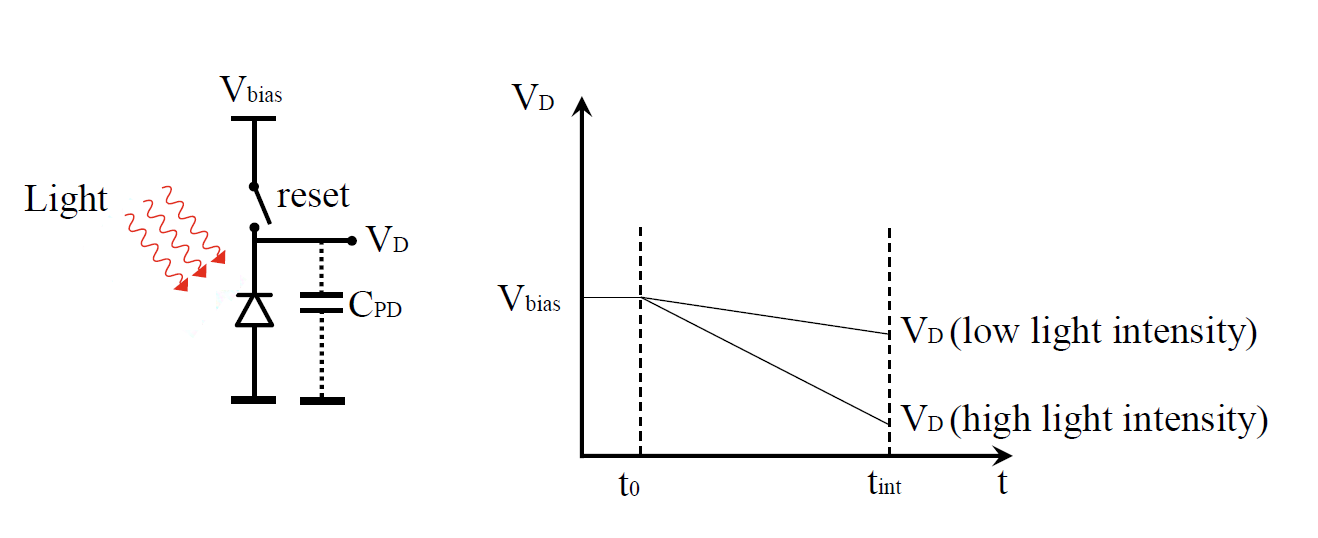
\includegraphics[width=\textwidth]{chapters/introduction/image/3T_pixel_readout.png} % Replace with your image
        \caption{}
        \label{}
    \end{subfigure}

    % Caption for the whole figure
    \caption[Cross-section and operation of an image sensor with 3T pixel architecture.]{(a) Schematic illustration of PePD integration on top of ROIC with 3T pixel architecture. Adapted from \cite{Kim2022DetailedSensors}. (b) Simplified schematic illustration of the 3T pixel architecture (left) and demonstration of bias signal variation during the signal integration period (right). Reproduced from \cite{Pejovic2023ColloidalInfrared}.}
    \label{fig:ch1:cmos_roic}
\end{figure}



The metrics related to the electrical performance of the developed PePD are largely defined by the architecture of the active pixel sensor (APS). In the scope of this work, and for prototyping reasons, we consider the use of a 3T pixel architecture that has been developed internally and has been repeatedly used to demonstrate imagers based on perovskite, organic, and quantum dot absorbers \cite{Song2024Lead-FreeSensors, Pejovic2021Thin-FilmImaging, Song2024HalideImager, Siddik2023Interface-EngineeredApplications}. Although the demonstration of a complete image sensor falls outside the scope of this work, understanding the operation of the APS is crucial for defining the performance requirements of the developed PePD. As the name indicates, the 3T pixel structure relies on the use of three transistors, namely the reset, the source follower and the row select transistor (Figure~\ref{fig:ch1:cmos_roic}a). A simplified schematic of the 3T pixel readout, as well as the variation of the voltage signal during a read-out cycle are shown in Figure~\ref{fig:ch1:cmos_roic}b. The read-out cycle is defined by the duration of the integration period ($t_{int}$). At the beginning of the integration period ($t_0$), the reset transistor is briefly turned-on, connecting the photodiode to a reference voltage in the reverse regime ($V_{bias}$). Next, the reset transistor is turned-off, however $V_{bias}$ is maintained across the photodiode, due to its internal capacitance ($C_{PD}$). During the integration period, and with the photodiode under illumination, the absorbed photons are converted to electron-hole pairs, which in turn discharge the diode's internal capacitance, effectively reducing the bias across its terminals. Therefore, at the end of the integration period, the bias across the diode ($V_D$) depends on the number of absorbed photons, i.e. the light intensity. As a last step, $V_D$ is buffered by the source follower transistor and processed by the rest of the circuit. 



As a result, during the read-out cycle, the PePD operates under a bias swing which is typically in the range of 100s mV to 1 V. During this bias swing, it is essential to ensure that the photoresponse of the PePD is independent of the bias point and that it depends solely on the intensity of the incoming light, thereby preserving output linearity. These requirements mean that it might be necessary to start the read-out cycle at higher reverse biases, in the range of -2 V, in contrary to the vast majority of published reports on PePDs, which typically limit the operation range to smaller biases, close to -0.5 V. The main disadvantage of operating at higher reverse bias is the associated increase in dark current, which inevitably lowers the signal-to-noise ratio and impairs the ability to detect weaker signals.


From the above, it becomes clear that the performance, scalability, and reliability requirements for the developed PePD create a set of conditions that are rarely considered simultaneously in published literature. To tackle all requirements and provide valuable insights into the development of reliable, vacuum-deposited, all-inorganic perovskite photodiodes the present thesis is structured as follows:  

\begin{itemize}

    \item Chapter~\ref{ch:material_properties} sets the foundations of using thermal co-evaporation for the deposition of \ch{CsPbI_2Br} thin films, while expanding on the experimental methodology followed throughout the thesis. Additionally, it highlights the sensitivity of characterization results to measurement settings, underscoring the need for careful and methodical interpretation of experimental data acquired from perovskite-based devices.

    \item Chapter~\ref{ch:ellipsometry} expands on a detailed, material-focused characterization of the thermally-evaporated \ch{CsPbI_2Br} thin films and evaluates the impact of the post-deposition thermal annealing step on their properties. In this context, spectroscopic ellipsometry is proposed as a versatile, easily accessible and non-destructive characterization technique that can be used to monitor the in situ annealing effect on \ch{CsPbI_2Br} thin films. A novel dynamic modeling approach of spectroscopic ellipsometry data is introduced, whose reliability is confirmed through additional characterization measurements or comparisons with literature. 

    \item Chapter~\ref{ch:transport_layer} covers everything related to the use of the \ch{CsPbI_2Br} thin films for the development of vacuum-deposited, all-inorganic photodiodes. After evaluating the impact of the perovskite deposition conditions (including the deposition rate, precursor stoichiometry, and annealing conditions), it proceeds to an extensive study on the impact of the electron transport layer on the reverse bias stability and response speed of the photodiode. Additionally, the high-temperature tolerance of the PePD is confirmed.

    \item  Lastly, Chapter~\ref{ch:stability} focuses on the phase stability of thermally evaporated \ch{CsPbI_2Br} thin films in ambient conditions. Once it is recognized that the lack of result-repeatability prevents the extraction of meaningful conclusions, a high-throughput, combinatorial experimentation approach is adopted, shedding light on the impact of precursor stoichiometry, perovskite thickness, and substrate type on the ambient stability of co-evaporated \ch{CsPbI_2Br} thin films. Finally, the tolerance of device performance for samples stored in ambient conditions is also evaluated. 
    
\end{itemize}







%%%%%%%%%%%%%%%%%%%%%%%%%%%%%%%%%%%%%%%%%%%%%%%%%%
% Keep the following \cleardoublepage at the end of this file, 
% otherwise \includeonly includes empty pages.
\cleardoublepage

% vim: tw=70 nocindent expandtab foldmethod=marker foldmarker={{{}{,}{}}}
